Obiettivo del controllo orbitale drag-free è la cancellazione delle forze non
gravitazionali agenti sul satellite per rendere il moto del centro di massa del
satellite dovuto con accettabile approssimazione esclusivamente alle forze
gravitazionali. L'accelerazione del centro di massa del satellite è descritta
dalle seguenti relazioni (tutte le coordinate sono espresse nel riferimento
corpo):

\begin{equation}
\components{\dot{v}}(t) = \components{g}(\components{r}(t))+
\frac{R_b(\quat{q})(-\components{F_d}(t)+\components{F_t}(t))}{m},
\components{v(0)=v_	0}
\end{equation}
dove $\components{F_d}$ sono le forze non gravitazionali (principalmente
aerodinamiche in orbita bassa) e $\components{F_t}$ sono le forze di comando
dovute ai propulsori.

Il controllo drag-free è soddisfatto quando la seguente relazione è soddisfatta:

\begin{equation}
\components{a}(t) = \frac{(- \components{F_d}(t) + \components{F_t}(t))}{m}=0
\end{equation}
ovvero l'accelerazione residua dovuta a componenti non gravitazionali
($\components{a}$) è nulla.

L'architettura prescelta per la compensazione delle forze suddette è basata 
sull' embedded model i cui concetti fondamentali sono:
\begin{description}
\item[Dinamica Controllabile:] Descrive la dinamica tra comando e misura, deve
catturare le dinamiche ad alta frequenza il più vicino possibile alla più alta
componente in frequenza dei disturbi da cancellare.
\item[Dinamica del Disturbo:] Dinamica rappresentante il disturbo e modellata su
base statistica.
\end{description} 

\begin{figure}
\includegraphics[page=13, trim=2.5cm 18.5cm 3cm 3cm,
clip=true,width=\textwidth]{control/orbit_control/images/cap7.pdf}
\caption{Architettura del controllo}
\end{figure}

